\documentclass[a4 paper, 10pt]{article}

\usepackage[latin1]{inputenc}
\usepackage[left=1in, right=1in]{geometry}
\usepackage{amsmath}
\usepackage{amsfonts}
\usepackage{amssymb}
\usepackage{amsthm}
\usepackage{setspace}\onehalfspacing
\usepackage{cases}
\AtBeginDocument{%
  \addtolength\abovedisplayskip{-0.5\baselineskip}%
  \addtolength\belowdisplayskip{-0.5\baselineskip}%
\addtolength\abovedisplayshortskip{-0.5\baselineskip}%
% \addtolength\belowdisplayshortskip{-0.5\baselineskip}%
}
\usepackage{enumitem}
\usepackage{color}
\usepackage{tikz}
\usetikzlibrary{graphs,arrows,decorations.pathmorphing,backgrounds,positioning,fit,chains,matrix,scopes,decorations.markings}
\usepackage{braids}
% Theorem Styles
\newtheorem{theorem}{Theorem}[section]
\newtheorem{conjecture}[theorem]{Conjecture}
\newtheorem{lemma}[theorem]{Lemma}
\newtheorem{proposition}[theorem]{Proposition}
\newtheorem{corollary}[theorem]{Corollary}
\newtheorem{case}{Case}
% Definition Styles
\theoremstyle{definition}
\newtheorem{definition}{Definition}[section]
\newtheorem{example}{Example}[section]
\theoremstyle{remark}
\newtheorem{remark}{Remark}
\setlength{\parindent}{0pt}
\linespread{1.0}
\newcommand{\Tone}{\mathcal{T}_1}
\newcommand{\Ttwo}{\mathcal{T}_2}
\newcommand{\C}{\mathbb{C}}
\newcommand{\sln}{\mathfrak{sl}_{n+1}(\C)}
\newcommand{\fg}{\mathfrak{g}}
\newcommand{\fk}{\mathfrak{k}}
\newcommand{\Ads}{\text{Ad}(s)}
\newcommand{\Adwx}{\text{Ad}(w_X)}
\newcommand{\Adsi}{\text{Ad}(s_i)}
\newcommand{\Ug}{U_q(\mathfrak{g})}
\newcommand{\Uk}{U'_q(\mathfrak{k})}
\newcommand{\qm}{q-q^{-1}}
\newcommand{\Acc}{\mathcal{A}_{\mathbf{c},\mathbf{c}^{\prime}}}
\newcommand{\qp}{q+q^{-1}}
\newcommand{\qqq}{[B_1,[B_2,[F_3,B_4]_{q}]_{q}]_{q}}
\newcommand{\ppp}{[B_5,[B_4,[F_3,B_2]_{q}]_{q}]_{q}}
\newcommand{\comm}[3]{[#1,#2]_{#3}}
\newcommand{\T}[1]{\mathcal{T}_{#1}}
\newcommand{\Bcc}{B_{\mathbf{c}}}
\newcommand{\cosub}{\overset{\scriptscriptstyle 1}{\subset}}
\newcommand{\cosup}{\overset{\scriptscriptstyle 1}{\supset}}
\newcommand{\Vpair}{(V,V^{\prime})}


\newcommand{\lequals}{\mathbin{\rotatebox[origin = c]{90}{$\equal$}}}
\numberwithin{equation}{section}

\begin{document}
\title{Current progress with calculating quasi K-matrices for coideal subalgebras}
\date{}
\maketitle

This is just a case-by-case summary of what we have calculated so far. In general, we have a set $I$ corresponding to nodes of the corresponding Dynkin diagram, a subset $X$ of black nodes and a diagram automorphism $\tau$.

\subsection{Type $A_n$ with non-trivial $\tau$ and $X = \{2,...,n-1\}$}
The picture in this case looks like the following.

\begin{center}
	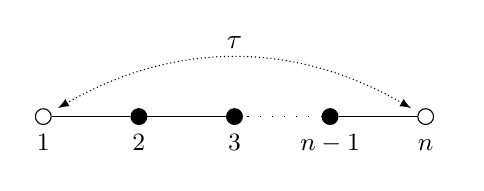
\begin{tikzpicture}  %would be nice to do this fully for any number of dots
		[white/.style={circle,draw=black,inner sep = 0mm, minimum size = 2mm},
		black/.style={circle,draw=black,fill=black, inner sep= 0mm, minimum size = 2mm}]
	
		\node[white] (first) [label = below:{\small $1$}] {};
		\node[black] (second) [right=of first] [label = below:{\small $2$}] {}
			edge (first);
		\node[black] (third) [right=of second] [label = below:{\small $3$}] {}
			edge (second);
		\node[black] (last) [right=of third] [label = below:{\small $n-1$}] {}
			edge [loosely dotted] (third);		
		\node[white] (fourth) [right=of last] [label = below:{\small $\phantom{0}n\phantom{0}$}] {}
			edge (last)
			edge	 [latex-latex , shorten <=3pt, shorten >=3pt, bend right=30, densely dotted] node[auto,swap] {$\tau$} (first); %probably change the arrow
	\end{tikzpicture}
\end{center}

Note that in the case where $I = \{1,2\}$, $X = \emptyset$ and there is no problem later on. 
Before we state what the quasi K-matrix in this case, we need to define some terms. We set
\begin{align*}
	b_i &:= \begin{cases}
	 			q^{i-1}[i]_q \qquad &\mbox{for $i \geq 1$,}\\
				1 \qquad &\mbox{for $i = 0$,}
			\end{cases}\\
	a_k^{(n)}&:=	\begin{cases}
					\dfrac{1}{b_n...b_1b_0} \qquad &\mbox{for $i = 0$ or $n$,}\\
					\dfrac{1}{(b_n...b_1b_0)(b_{n-k}...b_1b_0)} \qquad & \mbox{otherwise.}
				\end{cases}
\end{align*}

Observe that $a_{k}^{(n)} = a_0^{(n)}a_0^{(n-k)}$ for $k \neq 0$. This I believe will be useful soon.

Let $T_i$ denote the Lusztig automorphism corresponding to $i \in I$. We now define the following elements of $U^{+}$.
\begin{align*}
	X_{1;n-1} &:= T_{1--(n-2)}(E_{n-1}),\\
	X_{n;2} &:= T_{n--2}(E_1).
\end{align*}

Here, $T_{1--(n-2)}(E_{n-1})$ means calculating $T_1T_2...T_{n-2}(E_{n-1})$ and similarly for $T_{n--2}(E_1)$. A nice property of these two elements is that they commute.

The calculation that we have done tells us that

\begin{equation}
	\mathfrak{X} = \sum_{n \in \mathbb{N}} \sum_{k=0}^{n} a_k^{(n)}X_{1;n-1}^kX_{n;2}^{n-k}.
\end{equation}

The observation above allows us to rewrite this expression in the following way.

\begin{equation}
	\mathfrak{X} = (\sum_{k\geq 0} a_0^{(k)}X_{1;n-1}^k) (\sum_{k\geq 0} a_0^{(k)}X_{n;2}^k)
\end{equation}

\subsection{Type $A_n$ with identity diagram automorphism and $X$ empty}
In this case, we assume that the constants $s_i$ that appear when defining the coideal subalgebra are all zero. This simplifies matters massively. The picture we have for this case is the following.

\begin{center}
	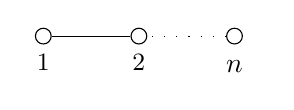
\begin{tikzpicture}  %would be nice to do this fully for any number of dots
		[white/.style={circle,draw=black,inner sep = 0mm, minimum size = 2mm},
		black/.style={circle,draw=black,fill=black, inner sep= 0mm, minimum size = 2mm}]
	
		\node[white] (first) [label = below:{\small $1$}] {};
		\node[white] (second) [right=of first] [label = below:{\small $2$}] {}
			edge (first);
		\node[white] (last) [right=of second] [label = below:{$\phantom{0}n\phantom{0}$}] {}
			edge [loosely dotted] (second);
	\end{tikzpicture}
\end{center}

Let $\mathfrak{X}_{1;(n-1)}$ denote the quasi K-matrix in rank $n-1$. Note that in the rank one case, we calculate that

\begin{equation}
	\mathfrak{X}_{1;1} = \sum_{k \geq 0} \dfrac{(q-q^{-1})^{k}(q^{2}c_1)^{k}}{b_{2k} \dots b_4b_2b_0} E_1^{2k}.
\end{equation}


An inductive argument then allows us to obtain
\begin{equation}
	\mathfrak{X}_{1;n} = \Big( \sum_{k_n \geq 0} \gamma_{k_n} E_n^{2k_n} \Big) \Big( \sum_{k_{n-1}\geq 0} \gamma_{k_{n-1}} T_{n-1}(E_n)^{2k_{n-1}} \Big) \dots \Big( \sum_{k_1 \geq 0} \gamma_{k_1} T_{1--(n-1)}(E_n)^{2k_1} \Big)\mathfrak{X}_{1;(n-1)}
\end{equation}
\\
where the coefficients $\gamma_{k_i}$ are given by 
\begin{equation}
	\gamma_{k_i} = \dfrac{(q-q^{-1})^{k_i}(q^{2(n-1+1)}c_i \dots c_n)^{k_i}}{b_{2k_i} \dots b_4b_2b_0}.
\end{equation}

Sometimes, it is more useful to give $\gamma_{k_i}$ in terms of the recurrence relation

\begin{equation}
	\gamma_{k_i} = \dfrac{(q-q^{-1})q^{2(n-1+1)}c_i \dots c_n}{b_{2k_i}}\gamma_{k_i-1}.
\end{equation}

An important point is that we only ever see even powers of the PBW basis elements appearing. This can be seen when looking at the expressions
\begin{align*}
	r_i(\mathfrak{X}_{\mu}) &= (q-q^{-1})\overline{c_i}\mathfrak{X}_{\mu - 2\alpha_i}E_i,\\
	_{i}r(\mathfrak{X}_{\mu}) &= (q-q^{-1})c_iE_i\mathfrak{X}_{\mu - 2\alpha_i}.
\end{align*}

Using this, it is clear in the rank one case that $\mathfrak{X}_{\mu}$ in non-zero if and only if $\mu = 2m\alpha_1$ for some $m \geq 0$.
We can build this reasoning inductively to conclude that we only obtain even powers.

\subsection{Type $A_3$ with identity diagram automorphism and $X = \{1,3\}$}
	We have the following diagram in this setting.
	
\begin{center}
	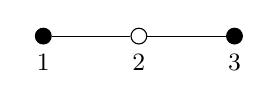
\begin{tikzpicture}  %would be nice to do this fully for any number of dots
		[white/.style={circle,draw=black,inner sep = 0mm, minimum size = 2mm},
		black/.style={circle,draw=black,fill=black, inner sep= 0mm, minimum size = 2mm}]
	
		\node[black] (first) [label = below:{\small $1$}] {};
		\node[white] (second) [right=of first] [label = below:{\small $2$}] {}
			edge (first);
		\node[black] (last) [right=of second] [label = below:{\small $3$}] {}
			edge (second);
	\end{tikzpicture}
\end{center}

In this case, we obtain

\begin{equation}
	\mathfrak{X} = \sum_{k \geq 0} \dfrac{(q-q^{-1})^kc_2^k}{b_k \dots b_2b_1b_0}\big(T_2(E_3)T_1(E_2) - q^{-1}T_1T_2(E_3)E_2\big)^k.
\end{equation}

The element inside the brackets can be rewritten to make symmetry clearer.

\begin{equation*}
	T_2(E_3)T_1(E_2) - q^{-1}T_1T_2(E_3)E_2 = \big[[E_2,E_3]_{q^{-1}}, E_1\big]_{q^{-1}}E_2 - q^{-1}T_2(E_3)T_2(E_1)
\end{equation*}

Somehow, I prefer the first expression so I want to keep with this where possible.

\newpage
\subsection{Type $B_2$ with identity diagram automorphism.}
We consider the following diagram.

\begin{center}
	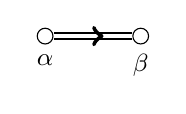
\begin{tikzpicture}[  %would be nice to do this fully for any number of dots
		white/.style={circle,draw=black,            inner sep= 0mm, minimum size = 2mm},
		black/.style={circle,draw=black,fill=black, inner sep= 0mm, minimum size = 2mm},
		B arrow/.style={
			thick,
			double distance=1.3pt,
			decoration={
				markings,
				mark=at position 0.51 with {\arrow[line width=1.6pt]{<}}
			},
			postaction=decorate
		}
	]
	
		\node[white] (first) [label = below:{\small $\alpha$}] {};
		\node[white] (second) [right=of first] [label = below:{\small $\beta$}] {}
			edge [B arrow] (first);
			
		
	\end{tikzpicture}
\end{center}

Here, $\alpha$ represents the long root and $\beta$ the short root. As with the previous cases, we see that we only consider even powers of the PBW-basis elements $E_{\alpha}, E_{\alpha + \beta}, E_{\alpha + 2\beta}$ and $E_{\beta}$. The main difference now is that the relations change, making this a much tougher calculation. Since we have a short root and a long root, we also have to be careful with $q$-powers. In particular, we have $q_{\alpha} = q^2$ and $q_{\beta} = q$. The coefficients $\gamma_i$ and $\mu_l$ below illustrate why these are important. We keep the notation $b_i$ as before but introduce new notation

\begin{equation*}
	a_i := 	\begin{cases}
				q_\alpha^{i-1}[i]_{q^2} = q^{2(i-1)}[i]_{\alpha} \qquad &\mbox{ if $i \geq 1$, }\\
				1 \qquad &\mbox{ if $ i = 0$.}
			\end{cases}
\end{equation*}

Then, after a long and involved calculation, we obtain

\begin{equation} \label{B2}
	\mathfrak{X} = \Big( \sum_{i \geq 0} \gamma_i E_{\beta}^{2i} \Big) \Big( \sum_{j \geq 0} \delta_j E_{\alpha + 2\beta}^{2j} \Big) \Big( \sum_{k \geq 0} \lambda_k E_{\alpha + \beta}^{2k} \Big) \Big( 							\sum_{l \geq 0} \mu_l E_{\alpha}^{2l} \Big)
\end{equation}

where the coefficients $\gamma_i, \delta_j, \lambda_k$ and $\mu_l$ are given by

\begin{align*}
	\gamma_i &= \dfrac{ ( q - q^{-1} )^i ( q^2 c_{\beta} )^i }{ b_{2i} \dots b_2 b_0 },\\ 		
	\delta_j &= \dfrac{ (q^2 - q^{-2})^j ( q^4 c_{\alpha} )^j ( q^4 c_{\beta}^2 )^j }{ a_{2j} \dots a_2 a_0 },\\
	\lambda_k &= \dfrac{( q - q^{-1} )^k ( q^4 c_{\alpha} )^k ( q^2 c_{\beta} )^k }{ b_{2k} \dots b_2 b_0 },\\		
	\mu_l &= \dfrac{ ( q^2 - q^{-2} )^l ( q^4 c_{\alpha} )^l }{ a_{2l} \dots a_2 a_0 }.
\end{align*}

This is a nice result, since it is exactly what one would expect given the previous calculations for type $A_n$ with identity diagram automorphism.
\section{Unfinished Cases}
Our next step, should be to look at the following three cases.

\begin{center}
	\begin{tikzpicture}  %would be nice to do this fully for any number of dots
		[white/.style={circle,draw=black,inner sep = 0mm, minimum size = 2mm},
		black/.style={circle,draw=black,fill=black, inner sep= 0mm, minimum size = 2mm}]
	
		\node[white] (first) [label = below:{\small $1$}] {};
		\node[white] (second) [right=of first] [label = below:{\small $2$}] {}
			edge (first);
		\node[white] (third) [right=of last] [label = below:{\small $3$}] {}
			edge (second)
			edge	 [latex-latex , shorten <=3pt, shorten >=3pt, bend right=30, densely dotted] node[auto,swap] {$\tau$} (first); %probably change the arrow
	\end{tikzpicture}
\hspace{1.5cm}		
	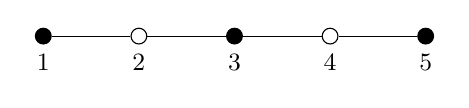
\begin{tikzpicture}  %would be nice to do this fully for any number of dots
		[white/.style={circle,draw=black,inner sep = 0mm, minimum size = 2mm},
		black/.style={circle,draw=black,fill=black, inner sep= 0mm, minimum size = 2mm}]
	
		\node[black] (first) [label = below:{\small $1$}] {};
		\node[white] (second) [right=of first] [label = below:{\small $2$}] {}
			edge (first);
		\node[black] (third) [right=of second] [label = below:{\small $3$}] {}
			edge (second);
		\node[white] (fourth) [right = of third] [label = below:{\small $4$}] {}
			edge (third);
		\node[black] (last) [right = of fourth] [label = below:{\small $5$}] {}
			edge (fourth);
	\end{tikzpicture}
\hspace{1.5cm}
	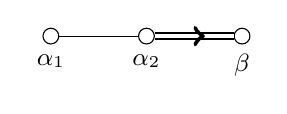
\begin{tikzpicture}[  %would be nice to do this fully for any number of dots
		white/.style={circle,draw=black,            inner sep= 0mm, minimum size = 2mm},
		black/.style={circle,draw=black,fill=black, inner sep= 0mm, minimum size = 2mm},
		B arrow/.style={
			thick,
			double distance=1.3pt,
			decoration={
				markings,
				mark=at position 0.51 with {\arrow[line width=1.6pt]{<}}
			},
			postaction=decorate
		}
	]
		\node[white] (first)[label = below:{\small $\alpha_1$}] {};
		\node[white] (second)[right=of first] [label = below:{\small $\alpha_2$}] {}
			edge (first);
		\node[white] (third) [right=of second] [label = below:{\small $\beta$}] {}
			edge [B arrow] (second);
			
		
	\end{tikzpicture}
\end{center}

I have looked a bit into the type $B_3$ calculation, but am currently stuck here. My feeling was that this would follow from the $B_2$ calculation but this does not seem to be the case.



\section{Type A3 with non-identity diagram automorphism}
We tackle the following case.

 \begin{center}
	\begin{tikzpicture}  %would be nice to do this fully for any number of dots
		[white/.style={circle,draw=black,inner sep = 0mm, minimum size = 2mm},
		black/.style={circle,draw=black,fill=black, inner sep= 0mm, minimum size = 2mm}]
	
		\node[white] (first) [label = below:{\small $1$}] {};
		\node[white] (second) [right=of first] [label = below:{\small $2$}] {}
			edge (first);
		\node[white] (third) [right=of last] [label = below:{\small $3$}] {}
			edge (second)
			edge	 [latex-latex , shorten <=3pt, shorten >=3pt, bend right=30, densely dotted] node[auto,swap] {$\tau$} (first); %probably change the arrow
	\end{tikzpicture}
\end{center}

We introduce the notion of an `admissible root' as an attempt of a generalisation of the previous cases. Let $\Theta = -w_X \circ \tau$. In this case, $w_X = \text{id}$. We call a root $\beta$ \emph{admissible} if $\beta \in \Phi^+ \cap \{ \alpha - \Theta(\alpha) | \alpha \in \Phi^+ \}$. In the present case, we see that there are no admissible roots. Admissible roots do exist in other cases. For example, in $A3$ with $X = \{2\} $, the root $\alpha_1 + \alpha_2 + \alpha_3$ is admissible.

We describe a potential algorithm for constructing the quasi K-matrix from a choice of longest word $w_0$. Let $w_0 = s_{i_1}s_{i_2} \dots s_{i_t}$. Then we construct a PBW basis $E_{\gamma_{i_1}}, E_{\gamma_{i_2}}, \dots, E_{\gamma_{i_t}}$ for $U^+(w_0)$ in the usual way by letting $E_{\gamma_{i_k}} = T_{i_1} \dots T_{i_{k-1}}(E_{i_k})$ for $k = 1, \dots, t$.

The algorithm goes as follows. We order the PBW basis elements as $E_{\gamma_{i_t}}, \dots, E_{\gamma_{i_1}}$. We go through each element and check if the underlying root is an admissible root or not. If it is then we obtain factors

\begin{equation}
	\big( \sum_{n} \alpha_{n}E_{\gamma_{i_k}^n} \big) \big( \sum_{m} \beta_{m}\tau(E_{\gamma_{i_k}}^m) \big).
\end{equation}  

If the underlying root $\beta$ is not admissible, then we check if $\beta - \Theta(\beta)$ is a positive simple root or not. If $\beta - \Theta(\beta)$ is not simple, then we obtain a factor

\begin{equation}
	\Big( \sum_{n} \gamma_{n} \big( E_{\gamma_{i_k}}\tau(E_{\gamma_{i_k}}) \big)^n \Big),
\end{equation}

otherwise, we completely omit $E_{\gamma_{i_k}}$. 

In the present case, if we choose $w_0 = s_1s_3s_2s_1s_3s_2$, then this algorithm does give us a factorized expression for the quasi K-matrix. In particular, we obtain

\begin{equation}
	\mathfrak{X} = \Big( \sum_{n_1} \alpha_{n_1} E_2^{2n_1} \Big) \Big( \sum_{n_2} \beta_{n_2} \big( T_3(E_2)T_1(E_2) \big)^{n_2} \Big) \Big( \sum_{n_3} \gamma_{n_3} T_1T_3(E_2)^{2n_3} \Big) \Big( \sum_{n_4} \delta_{n_4} \big( E_1E_3 \big)^{n_4} \Big) 
\end{equation}

where the coefficients $\alpha_{n_1}, \beta_{n_2}, \gamma_{n_3}, \delta_{n_4}$ are given by

\begin{align*}
	\alpha_{n_1} &= \dfrac{ ( q - q^{-1} )^{n_1} ( q^2 c_{2} )^{n_1} }{ \{2n_1\} \dots \{2\} \{0 \}},\\ 		
	\beta_{n_2} &= \dfrac{ (q - q^{-1})^{n_2} ( q^2 c_{2} )^{n_2}}{ \{n_2\}! },\\
	\gamma_{n_3} &= \dfrac{( q - q^{-1} )^{n_3} ( q^4 c_{2} )^{n_3} }{ \{2n_3\} \dots \{2\} \{0\} },\\		
	\delta_{n_4} &= \dfrac{ ( q - q^{-1} )^{n_4} }{ \{n_4\}! }.
\end{align*}

Perhaps interestingly, if we not take the word $w_0 = s_2s_1s_3s_2s_1s_3$, then we obtain a different factorization

\begin{equation}
	\mathfrak{X} = \Big( \sum_{n_1} \alpha^{\prime}_{n_1} \big( E_1E_3 \big)^{n_1} \Big) \Big( \sum_{n_2} \beta^{\prime}_{n_2} T_2T_1T_3(E_2)^{2n_2} \Big) \Big( \sum_{n_3} \gamma^{\prime}_{n_3}  \big( T_2(E_3)T_2(E_1) \big)^{n_3} \Big) \Big( \sum_{n_4} \delta^{\prime}_{n_4} E_2^{2n_4} \Big) 
\end{equation}

where 

\begin{equation*}
	\alpha_{n}^{\prime} = \delta_n, \qquad 		
	\beta_{n}^{\prime} = \gamma_n, \qquad
	\gamma_{n}^{\prime} = \beta_n, \qquad		
	\delta_{n}^{\prime} = \alpha_n.
\end{equation*}

One would hope that such a method will work independently of the representative of the longest word chosen. However, I believe this to not quite be the case. For example, if we choose $w_0 = s_1s_2s_1s_3s_2s_1$, then our current algorithm implies that the quasi K-matrix is of the form

\begin{equation}

\end{equation}
\end{document}